\documentclass[10pt]{article}
\usepackage{fancyhdr}
\usepackage{amsmath}
\usepackage{graphicx}
\pagestyle{fancy}
\headheight 35pt
\parskip 10pt \parindent 0pt 
\lhead{Classical Mechanics HW 2}
\chead{Andrei Ilyashenko}
\rhead{09-21-2010}
\cfoot{\thepage}

\begin{document}
%%%%%%%%%%%%%%%%%%%%%%%%%%%%%%%%%%%%%%%%%%%%%%%%%%%%%%%%%%%%%%%%%%%%%%%%%%%%%%%%%%%%
\textbf{Ex 12}\\
If, the Lagrangian depended on second derivatives of the coordinates, then when we vary it, we get
\begin{align*}
  \delta I &= \delta \int L(q_1, \dots q_n, \dot q_1 \dots \dot q_n, \ddot q_1 \dots \ddot q_n, t)dt.
\end{align*}
As usual, let the coordinates depend on $t$ and some parameter $\alpha_i$, 
such that $q_i(t,\alpha) = q_i(t,0) + \alpha \eta_i(t)$, and $q_i(t,0)$, 
is the solution that makes the action stationary.  Then, the variation of I 
is given by 
\begin{align*}
  \delta I &= \frac{\partial I}{\partial \alpha} = \int \sum_i \left(  \frac{\partial L}{\partial q_i}\frac{\partial q_i}{\partial \alpha} + \frac{\partial L}{\partial \dot q_i}\frac{\partial \dot q_i}{\partial \alpha} + \frac{\partial L}{\partial \ddot q_i}\frac{\partial \ddot q_i}{\partial \alpha} \right)dt
\end{align*}
We can integrate the second term by parts once, and the third term twice to 
get, 
\begin{align*}
  \delta I &= \left( \frac{\partial L}{\partial q_i}-\frac{d}{dt}\frac{\partial L}{\partial \dot q_i} + \frac{d^2}{dt^2}\frac{\partial L}{\partial \ddot q_i} \right) \frac{\partial q_i}{\partial \alpha}.
\end{align*}
The surface terms arising from the integration by parts go to zero, because 
there is no variation on the ends.  This is then set to zero, in order to 
find the solution that minimizes the action, and using the fundamental
lemma of the calculus of variations, we get
\begin{align*}
   \frac{\partial L}{\partial q_i}-\frac{d}{dt}\frac{\partial L}{\partial \dot q_i} + \frac{d^2}{dt^2}\frac{\partial L}{\partial \ddot q_i} &= 0,
\end{align*}
as expected.  Now, if $L=-(m/2)q\ddot q - (k/2) q^2$, then we get
\begin{align*}
  -\frac{m}{2}\ddot q -kq -\frac{d}{dt}0 + \frac{d^2}{dt^2}'\left(\frac{m}{2}q  \right) &= 0,
\end{align*}
and if the mass is constant, this becomes,
\begin{align*}
  m\ddot q = -kq,
\end{align*}
the equation for the 1D spring obeying Hooke's law.\\
\textbf{Ex 14}\\
\begin{figure}[h!]
    \centering
    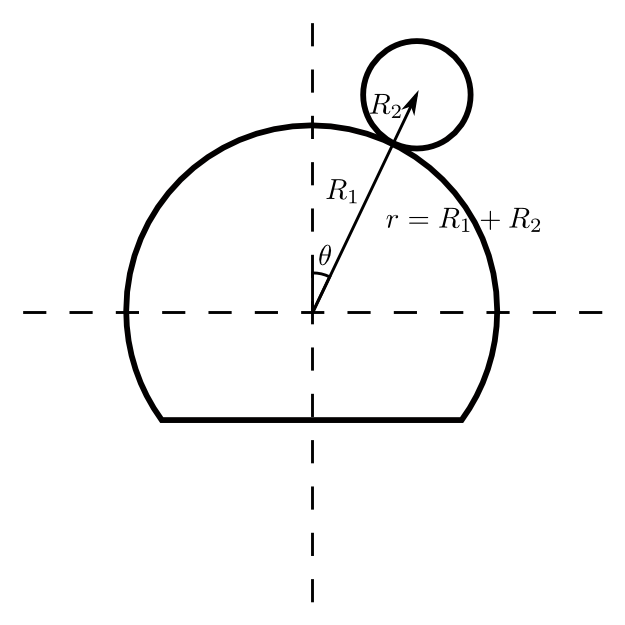
\includegraphics[width=0.7\textwidth]{Ex14.png}
    \caption{A graph showing the generalized coordinates $r$, and $\theta$.  The uniform hoop of mass $m$ and radius $R_2$ rolls without slipping on the surface of the fixed cylinder of radius $R_2$.}
  \label{fig:ex14}
\end{figure}
Fig. \ref{fig:ex14} shows the coordinate system. In order to simplify 
the notation $R_c$ is the constant radius of the cylinder, $R_h$ is the 
constant radius of the hoop, and $r$ is a generalized coordinate specifying 
the distance between the hoop and the cylinder.  There are two
constraints, one is that the hoop does not slip, which can be written 
as $R_2^2\omega^2 = (r-R_2)^2\dot\theta^2 + \dot r^2$.  Since we are
not asked to determine the force of constrain associated with this
constraint (friction), we will not incorporate this constraint using a
Lagrange multiplier, but rather we will let the choice of generalized 
coordinates take care of it.  The second constraint, the that the hoop 
rolls along the cylinder, which can be written as $r = R_1+R_2$.  So, our 
Lagrangian is
\begin{align*}
  L' &= \frac{1}{2}I\omega^2 + \frac{1}{2}mv^2 - mgr\cos\theta + \lambda(r-R_1-R_2)\\
  L' &= \frac{1}{2}m((r-R_2)^2\dot\theta^2 + \dot r^2) + \frac{1}{2}m(\dot r^2+r^2\dot\theta^2) - mgr\cos\theta + \lambda(r-R_1-R_2)\\
\end{align*}
Now, we can find the equation of motion for $r$, and from that get an expression for $\lambda$
\begin{align}
  m(r-R_2)\dot\theta^2 + mr\dot\theta^2-mg\cos\theta + \lambda &= 0\nonumber\\
  m(2r-R_2)\dot\theta^2 - mg\cos\theta + \lambda &= 0\nonumber\\
  m(2R_1+R_2)\dot\theta^2 - mg\cos\theta + \lambda &= 0,\label{eq:ex14Constraint}
\end{align}
note that all terms involving $\dot r$ have been dropped since $r=R_1+R_2$.  
Now, we need an expression for $\dot\theta^2$ in terms of $\theta$, 
we get this from conservation of energy, and for conciseness, the constraint
$r=R_1+R_2$ is applied to eliminate $r$.  The initial energy of the system is
$mg(R_1+R_2)$, since initially, the system is at rest on top of the cylinder,
thus
\begin{align*}
  \frac{1}{2}mR_1\dot\theta^2 + \frac{1}{2}m\left( (R_1+R_2)^2\dot\theta^2 \right) + mg(R_1+R_2)\cos\theta &= mg(R_1+R_2)\\
  \dot\theta^2 &= (1-\cos\theta)\frac{2g(R_1+R_2)}{(R_1+R_2)^2+R_1^2}\\
  \dot\theta^2 &= (1-\cos\theta)\frac{Ag}{2R_1+R_2}.
\end{align*}
Where $A$ is $2(R_1+R_2)(2R_1+R_2)/\left( (R_1+R_2)^2+R_1^2 \right)$.  Now 
substituting this expression into eq. \ref{eq:ex14Constraint}, gives
\begin{align*}
  \lambda &= mg(\cos\theta - A(1-\cos\theta))\\
  \lambda &= mg((A+1)\cos\theta-A).
\end{align*}
The hoop will fall off once the constraint force becomes 0, so
\begin{align*}
  0 &= ((A+1)\cos\theta-A)\\
  \cos\theta = \frac{A}{A+1}.
\end{align*}
Notice that the hoop was instead a point mass (ie $R_2=0$), then we get
\begin{align*}
  \cos\theta = \frac{2}{3},
\end{align*}
which is the result that we got in class for the point mass.

\textbf{Ex 16}\\
The equations of motion for the Lagrangian 
\begin{align*}
  L &= e^{yt}\left( m\frac{\dot q^2}{2}-\frac{kq^2}{2} \right)
\end{align*}
are
\begin{align*}
  -e^{yt}kq - \frac{d}{dt}(e^{yt} m\dot q)=0,
\end{align*}
and if $\dot m=0$, this becomes
\begin{align*}
  e^{yt}\left( -kq-ym\dot q-m\ddot q \right) &= 0.
\end{align*}
So, $m\ddot q = -kq-ym\dot q$, which means there are tow forces:
the force of friction $-ym\dot q$, and the spring force $-kq$.
So this is a damped 1D oscillator, or a 1D oscillator with friction
The energy function for this Lagrangian is
\begin{align*}
  h &= \dot q\frac{\partial L}{\partial \dot q}-L\\
    &= e^{yt}\left( \frac{m\dot q^2}{2}+\frac{kq^2}{2} \right)\\
    &= e^{yt}\left( T+V \right),
\end{align*}
where $T$ is the kinetic, and $V$ is the potential energy.  Since this function
depends explicitly on time, it is not conserved.  In fact, we know that
\begin{align*}
  \frac{dh}{dt} &= -\frac{\partial L}{\partial t}\\
  ye^{yt}\left( T+V \right) +e^{yt}\frac{d}{dt}\left( T+V \right)  &= -ye^{ty}\left( T-V \right)\\
  \frac{dE}{dt} &= -2yT\\
  \frac{dE}{dt} &= -ym\dot q^2.
\end{align*}
So, the energy is not conserved, but it dissipated by the second force 
(other than $-kq$).\\
Under the point transformation described in the book, the Lagrangian becomes
\begin{align*}
  L &= e^{-yt}\left( m\frac{(\dot s -ys)^2}{2}-\frac{ks^2}{2} \right),
\end{align*}
and the equations of motion are
\begin{align*}
  e^{-yt}\left( -ym(\dot s-ys)-ks \right) - \frac{d}{dt}\left( e^{-yt}m\dot s \right) &= 0\\
  e^{-yt}\left( -ym(\dot s-ys)-ks \right) +  ye^{-yt}m\dot s - e^{-yt}m\ddot s &= 0\\
  e^{-yt}\left( (y^2m-k)s - m\ddot s \right)  &= 0.
\end{align*}

\textbf{Ex 17}\\
If, we are able to write the kinetic and potential energy terms as
\begin{align*}
  T=\sum_if_i(q_i)\dot q_i^2 && V = \sum_iV_i(q_i)
\end{align*}
Then, the equations of motion becomes
\begin{align*}
  \frac{\partial L}{\partial q_i} - \frac{d}{dt}\left( \frac{\partial L}{\partial \dot q_i} \right) &= 0\\
  \frac{\partial f_i(q_i)}{\partial q_i}\dot q_i^2 - \frac{\partial V_i(q_i)}{\partial q_i} - \frac{d}{dt}\left( 2f_i(q_i)\dot q_i \right) &= 0\\
  -\frac{\partial f_i(q_i)}{\partial q_i}\dot q_i^2 - \frac{\partial V_i(q_i)}{\partial q_i} - 2f_i(q_i)\ddot q_i &= 0
\end{align*}
All other terms in the sum disappear because the other terms don't depend on 
$q_i$, so the partial differentiation yields 0.  Thus, the terms separate into
$i$ ODEs.
\textbf{Ex 20}\\
Let, $x$, and $y$ specify the position of the mass $m$, with $y$ being 
vertical and $x$ being horizontal, and the $x_w$ be the position of the
end of the wedge.  Thus the constraint is $(x-x_w)\tan\alpha - y = 0$, 
and the Lagrangian is
\begin{align*}
  L &= \frac{1}{2}\left( M\dot x_w^2 + m(\dot x^2+\dot y^2) \right)-mgy+\lambda(x-x_w-y\cot\alpha).
\end{align*}
The equations of motion arising from this Lagrangian are
\begin{align*}
  m\ddot x - \lambda &= 0\\
  m\ddot y + mg + \lambda\cot\alpha &= 0\\
  M\ddot x_w + \lambda &= 0\\
  \lambda &= m\ddot x = -M\ddot x_w.
\end{align*}
If we differentiate the constraint equation twice with respect to time, we get
$\ddot y = (\ddot x-\ddot x_w)\tan\alpha$, which is the same as 
$m\ddot y = (\lambda+\lambda/M)\tan\alpha$.  Substituting this expression into
the equation of motion for $y$ gives
\begin{align*}
  \lambda\left(\frac{M+m}{M}\right)\tan\alph + mg + \lambda\cot\alpha &= 0\\
  \lambda &= \frac{-mg}{\left( \frac{M+m}{M} \right)\tan\alpha+\cot\alpha}.
\end{align*}
So, the forces of constraint are 
\begin{align*}
  Q_x &= \lambda\\
  Q_y &= -\tan\alpha\lambda\\
  Q_{x_w} &= -\lambda.
\end{align*}
In time $t$, these force do work
\begin{align*}
  dW &= -\lambda dx_w + \lambda dx - \lambda\tan\alpha dy\\
  \int_0^t \dot W dt = \int_0^t\left( -\lambda \dot x_w + \lambda \dot x - \lambda\tan\alpha \dot y \right)dt\\
  W &= -\lambda (x_w(t)-x_w(0)) + \lambda \dot (x(t)-x(0)) - \lambda\tan\alpha (y(t)-y(0))\\
  W &= \lambda\left(  - (x_w(t)-x_w(0)) +  \dot (x(t)-x(0)) - \tan\alpha (y(t)-y(0)) \right)\\
  W &= 0,
\end{align*}
where in the second to last step I used the constraint equation.  So, the 
forces of constraint do no work.  One of the constants of motion, will be
the energy function, which in this case is just the total energy.
\begin{align*}
  E = \frac{1}{2}\left( M\dot x_w^2 + m(\dot x^2+\dot y^2) \right)+mgy.
\end{align*}



\end{document}
